% Options for packages loaded elsewhere
\PassOptionsToPackage{unicode}{hyperref}
\PassOptionsToPackage{hyphens}{url}
%
\documentclass[
  ignorenonframetext,
]{beamer}
\usepackage{pgfpages}
\setbeamertemplate{caption}[numbered]
\setbeamertemplate{caption label separator}{: }
\setbeamercolor{caption name}{fg=normal text.fg}
\beamertemplatenavigationsymbolsempty
% Prevent slide breaks in the middle of a paragraph
\widowpenalties 1 10000
\raggedbottom
\setbeamertemplate{part page}{
  \centering
  \begin{beamercolorbox}[sep=16pt,center]{part title}
    \usebeamerfont{part title}\insertpart\par
  \end{beamercolorbox}
}
\setbeamertemplate{section page}{
  \centering
  \begin{beamercolorbox}[sep=12pt,center]{section title}
    \usebeamerfont{section title}\insertsection\par
  \end{beamercolorbox}
}
\setbeamertemplate{subsection page}{
  \centering
  \begin{beamercolorbox}[sep=8pt,center]{subsection title}
    \usebeamerfont{subsection title}\insertsubsection\par
  \end{beamercolorbox}
}
\AtBeginPart{
  \frame{\partpage}
}
\AtBeginSection{
  \ifbibliography
  \else
    \frame{\sectionpage}
  \fi
}
\AtBeginSubsection{
  \frame{\subsectionpage}
}
\usepackage{amsmath,amssymb}
\usepackage{iftex}
\ifPDFTeX
  \usepackage[T1]{fontenc}
  \usepackage[utf8]{inputenc}
  \usepackage{textcomp} % provide euro and other symbols
\else % if luatex or xetex
  \usepackage{unicode-math} % this also loads fontspec
  \defaultfontfeatures{Scale=MatchLowercase}
  \defaultfontfeatures[\rmfamily]{Ligatures=TeX,Scale=1}
\fi
\usepackage{lmodern}
\ifPDFTeX\else
  % xetex/luatex font selection
\fi
% Use upquote if available, for straight quotes in verbatim environments
\IfFileExists{upquote.sty}{\usepackage{upquote}}{}
\IfFileExists{microtype.sty}{% use microtype if available
  \usepackage[]{microtype}
  \UseMicrotypeSet[protrusion]{basicmath} % disable protrusion for tt fonts
}{}
\makeatletter
\@ifundefined{KOMAClassName}{% if non-KOMA class
  \IfFileExists{parskip.sty}{%
    \usepackage{parskip}
  }{% else
    \setlength{\parindent}{0pt}
    \setlength{\parskip}{6pt plus 2pt minus 1pt}}
}{% if KOMA class
  \KOMAoptions{parskip=half}}
\makeatother
\usepackage{xcolor}
\newif\ifbibliography
\usepackage{color}
\usepackage{fancyvrb}
\newcommand{\VerbBar}{|}
\newcommand{\VERB}{\Verb[commandchars=\\\{\}]}
\DefineVerbatimEnvironment{Highlighting}{Verbatim}{commandchars=\\\{\}}
% Add ',fontsize=\small' for more characters per line
\usepackage{framed}
\definecolor{shadecolor}{RGB}{248,248,248}
\newenvironment{Shaded}{\begin{snugshade}}{\end{snugshade}}
\newcommand{\AlertTok}[1]{\textcolor[rgb]{0.94,0.16,0.16}{#1}}
\newcommand{\AnnotationTok}[1]{\textcolor[rgb]{0.56,0.35,0.01}{\textbf{\textit{#1}}}}
\newcommand{\AttributeTok}[1]{\textcolor[rgb]{0.13,0.29,0.53}{#1}}
\newcommand{\BaseNTok}[1]{\textcolor[rgb]{0.00,0.00,0.81}{#1}}
\newcommand{\BuiltInTok}[1]{#1}
\newcommand{\CharTok}[1]{\textcolor[rgb]{0.31,0.60,0.02}{#1}}
\newcommand{\CommentTok}[1]{\textcolor[rgb]{0.56,0.35,0.01}{\textit{#1}}}
\newcommand{\CommentVarTok}[1]{\textcolor[rgb]{0.56,0.35,0.01}{\textbf{\textit{#1}}}}
\newcommand{\ConstantTok}[1]{\textcolor[rgb]{0.56,0.35,0.01}{#1}}
\newcommand{\ControlFlowTok}[1]{\textcolor[rgb]{0.13,0.29,0.53}{\textbf{#1}}}
\newcommand{\DataTypeTok}[1]{\textcolor[rgb]{0.13,0.29,0.53}{#1}}
\newcommand{\DecValTok}[1]{\textcolor[rgb]{0.00,0.00,0.81}{#1}}
\newcommand{\DocumentationTok}[1]{\textcolor[rgb]{0.56,0.35,0.01}{\textbf{\textit{#1}}}}
\newcommand{\ErrorTok}[1]{\textcolor[rgb]{0.64,0.00,0.00}{\textbf{#1}}}
\newcommand{\ExtensionTok}[1]{#1}
\newcommand{\FloatTok}[1]{\textcolor[rgb]{0.00,0.00,0.81}{#1}}
\newcommand{\FunctionTok}[1]{\textcolor[rgb]{0.13,0.29,0.53}{\textbf{#1}}}
\newcommand{\ImportTok}[1]{#1}
\newcommand{\InformationTok}[1]{\textcolor[rgb]{0.56,0.35,0.01}{\textbf{\textit{#1}}}}
\newcommand{\KeywordTok}[1]{\textcolor[rgb]{0.13,0.29,0.53}{\textbf{#1}}}
\newcommand{\NormalTok}[1]{#1}
\newcommand{\OperatorTok}[1]{\textcolor[rgb]{0.81,0.36,0.00}{\textbf{#1}}}
\newcommand{\OtherTok}[1]{\textcolor[rgb]{0.56,0.35,0.01}{#1}}
\newcommand{\PreprocessorTok}[1]{\textcolor[rgb]{0.56,0.35,0.01}{\textit{#1}}}
\newcommand{\RegionMarkerTok}[1]{#1}
\newcommand{\SpecialCharTok}[1]{\textcolor[rgb]{0.81,0.36,0.00}{\textbf{#1}}}
\newcommand{\SpecialStringTok}[1]{\textcolor[rgb]{0.31,0.60,0.02}{#1}}
\newcommand{\StringTok}[1]{\textcolor[rgb]{0.31,0.60,0.02}{#1}}
\newcommand{\VariableTok}[1]{\textcolor[rgb]{0.00,0.00,0.00}{#1}}
\newcommand{\VerbatimStringTok}[1]{\textcolor[rgb]{0.31,0.60,0.02}{#1}}
\newcommand{\WarningTok}[1]{\textcolor[rgb]{0.56,0.35,0.01}{\textbf{\textit{#1}}}}
\usepackage{longtable,booktabs,array}
\usepackage{calc} % for calculating minipage widths
\usepackage{caption}
% Make caption package work with longtable
\makeatletter
\def\fnum@table{\tablename~\thetable}
\makeatother
\usepackage{graphicx}
\makeatletter
\newsavebox\pandoc@box
\newcommand*\pandocbounded[1]{% scales image to fit in text height/width
  \sbox\pandoc@box{#1}%
  \Gscale@div\@tempa{\textheight}{\dimexpr\ht\pandoc@box+\dp\pandoc@box\relax}%
  \Gscale@div\@tempb{\linewidth}{\wd\pandoc@box}%
  \ifdim\@tempb\p@<\@tempa\p@\let\@tempa\@tempb\fi% select the smaller of both
  \ifdim\@tempa\p@<\p@\scalebox{\@tempa}{\usebox\pandoc@box}%
  \else\usebox{\pandoc@box}%
  \fi%
}
% Set default figure placement to htbp
\def\fps@figure{htbp}
\makeatother
\setlength{\emergencystretch}{3em} % prevent overfull lines
\providecommand{\tightlist}{%
  \setlength{\itemsep}{0pt}\setlength{\parskip}{0pt}}
\setcounter{secnumdepth}{-\maxdimen} % remove section numbering
\usepackage{booktabs}
\usepackage{longtable}
\usepackage{array}
\usepackage{multirow}
\usepackage{wrapfig}
\usepackage{float}
\usepackage{colortbl}
\usepackage{pdflscape}
\usepackage{tabu}
\usepackage{threeparttable}
\usepackage{threeparttablex}
\usepackage[normalem]{ulem}
\usepackage{makecell}
\usepackage{xcolor}
\usepackage{bookmark}
\IfFileExists{xurl.sty}{\usepackage{xurl}}{} % add URL line breaks if available
\urlstyle{same}
\hypersetup{
  pdftitle={Module 2: MULTIPLE LINEAR REGRESSION Week 1},
  pdfauthor={Mette Langaas, Department of Mathematical Sciences, NTNU -- with contributions from Øyvind Bakke and Ingeborg Hem},
  hidelinks,
  pdfcreator={LaTeX via pandoc}}

\title{Module 2: MULTIPLE LINEAR REGRESSION Week 1}
\subtitle{TMA4315 Generalized linear models H2018}
\author{Mette Langaas, Department of Mathematical Sciences, NTNU -- with
contributions from Øyvind Bakke and Ingeborg Hem}
\date{30.08 and 06.09 {[}PL{]}, 31.08 and 07.09 {[}IL{]}}

\begin{document}
\frame{\titlepage}

\begin{frame}{Overview}
\phantomsection\label{overview}
\begin{block}{Learning material}
\phantomsection\label{learning-material}
\begin{itemize}
\tightlist
\item
  Textbook: Chapter 2.2, 3 and B.4.
\item
  \href{https://www.math.ntnu.no/emner/TMA4315/2018h/TMA4315M2H20180830.pdf}{Classnotes
  30.08.2018}
\item
  \href{https://www.math.ntnu.no/emner/TMA4315/2018h/TMA4315M2H20180906.pdf}{Classnotes
  06.09.2018}
\end{itemize}
\end{block}
\end{frame}

\begin{frame}
\begin{block}{Topics}
\phantomsection\label{topics}
\begin{block}{\hyperlink{firstweek}{First week}}
\phantomsection\label{first-week}
\begin{itemize}
\tightlist
\item
  Aim of multiple linear regression.
\item
  Define and understand the multiple linear regression model -
  traditional and GLM way
\item
  parameter estimation with maximum likelihood (and least squares)
\item
  likelihood, score vector and Hessian (observed Fisher information
  matrix)
\item
  big data implementation (if time)
\item
  properties of parameter estimators
\item
  assessing model fit (diagnostic), residuals, QQ-plots
\item
  design matrix: how to code categorical covariates (dummy or effect
  coding), and how to handle interactions
\end{itemize}
\end{block}
\end{block}
\end{frame}

\begin{frame}
\begin{block}{\hyperlink{secondweek}{Second week}}
\phantomsection\label{second-week}
\begin{itemize}
\tightlist
\item
  What did we do last week?
\item
  Statistical inference for parameter estimates

  \begin{itemize}
  \tightlist
  \item
    confidence intervals,
  \item
    prediction intervals,
  \item
    hypothesis test,
  \item
    linear hypotheses
  \end{itemize}
\item
  analysis of variance decompositions and \(R^2\), sequential ANOVA
  table
\item
  DEVIANCE???
\item
  model selection with AIC and variants
\end{itemize}
\end{block}
\end{frame}

\begin{frame}{Aim of multiple linear regression}
\phantomsection\label{aim-of-multiple-linear-regression}
\begin{enumerate}
\item
  \textbf{Explanation} Construct a model to help understand the
  relationship between a response and one or several explanatory
  variables.
\item
  \textbf{Prediction} Construct a model to predict the response from a
  set of (one or several) explanatory variables.
\end{enumerate}
\end{frame}

\begin{frame}[fragile]
\begin{block}{Munich rent index}
\phantomsection\label{munich-rent-index}
Munich, 1999: 3082 observations on 9 variables.

Interested in \texttt{rent}. Govt wants to know what a typical rent is
in different areas of Munich

\begin{itemize}
\tightlist
\item
  what variables explain it
\item
  how well can we predict it?
\end{itemize}

More information in Fahrmeir et. al., (2021) page 6.
\end{block}
\end{frame}

\begin{frame}[fragile]
\begin{block}{Munich rent index Variables}
\phantomsection\label{munich-rent-index-variables}
\begin{itemize}
\tightlist
\item
  \texttt{rent}: the net rent per month (in Euro).
\item
  \texttt{rentsqm}: the net rent per month per square meter (in Euro).
\item
  \texttt{area}: Living area in square meters.
\item
  \texttt{yearc}: year of construction.
\item
  \texttt{location}: quality of location: a factor indicating whether
  the location is average location, 1, good location, 2, and top
  location, 3.
\item
  \texttt{bath}: quality of bathroom: a a factor indicating whether the
  bath facilities are standard, 0, or premium, 1.
\item
  \texttt{kitchen}: Quality of kitchen: 0 standard 1 premium.
\item
  \texttt{cheating}: central heating: a factor 0 without central
  heating, 1 with central heating.
\item
  \texttt{district}: District in Munich.
\end{itemize}
\end{block}
\end{frame}

\begin{frame}
\pandocbounded{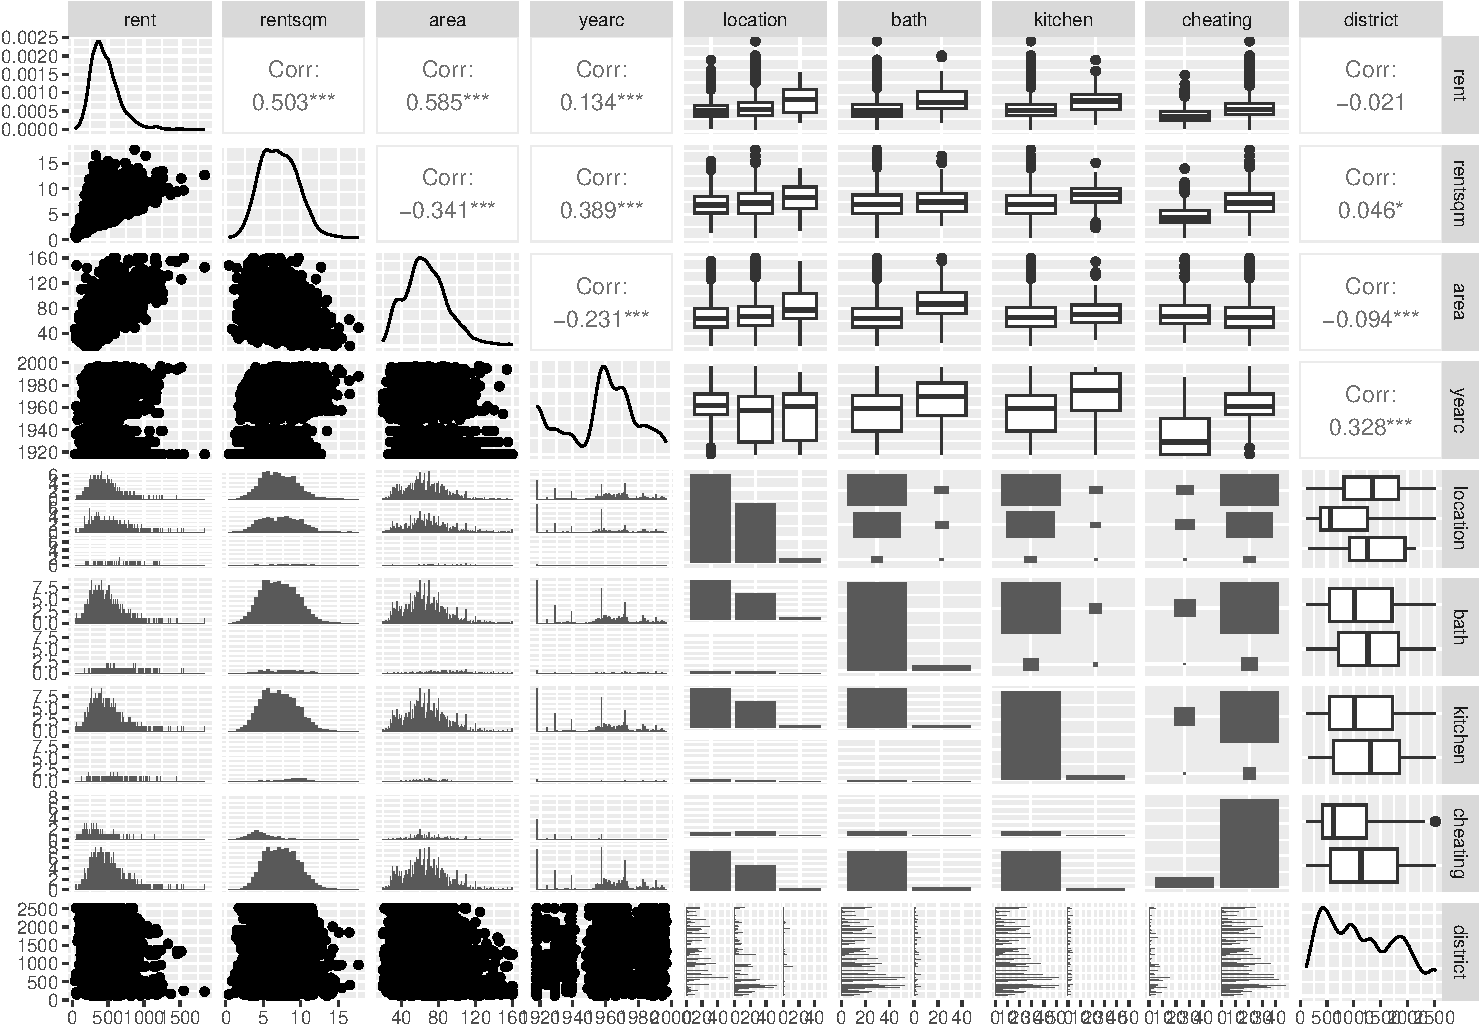
\includegraphics[keepaspectratio]{Module02MLRPresentationWeek1_files/figure-beamer/unnamed-chunk-1-1.pdf}}
\end{frame}

\begin{frame}[fragile]
\textbf{Interesting questions}

\begin{enumerate}
\tightlist
\item
  Is there a relationship between \texttt{rent} and \texttt{area}?
\item
  How strong is this relationship?
\item
  Is the relationship linear?
\item
  Are also other variables associated with \texttt{rent}?
\item
  How well can we predict the rent of an apartment?
\item
  Is the effect of \texttt{area} the same on \texttt{rent} for
  apartments at average, good and top \texttt{location}? (interaction)
\end{enumerate}
\end{frame}

\begin{frame}{Notation}
\phantomsection\label{notation}
\({\bf Y}: (n \times 1)\) vector of responses (random variable)
{[}e.g.~one of the following: rent, rent pr sqm, weight of baby, ph of
lake, volume of tree{]}

\({\bf X}: (n \times p)\) design matrix {[}e.g.~location of flat,
gestation age of baby, chemical measurement of the lake, height of
tree{]}

\(\boldsymbol{\beta}: (p \times 1)\) vector of regression parameters
(intercept included, so \(p=k+1\))

\(\boldsymbol{\varepsilon}: (n\times 1)\) vector of random errors. Used
in ``traditional way''.

We assume that pairs \(({\bf x}_i^T,y_i)\) (\(i=1,...,n\)) are measured
from sampling units. That is, the observation pair \(({\bf x}_1^T,y_1)\)
is independent from \(({\bf x}_2^T,y_2)\), and so on.
\end{frame}

\begin{frame}[fragile]
\begin{block}{Hands on: Munich rent index --- response and covariates}
\phantomsection\label{hands-on-munich-rent-index-response-and-covariates}
From the list of variable and the statement of the questions, answer
these questions:

\begin{itemize}
\tightlist
\item
  {What can be response, and what covariates? (using what you know about
  rents)}
\item
  {What type of response(s) do we have? (continuous, categorical,
  nominal, ordinal, discrete, factors, \ldots). }
\item
  {What types of covariates? (continuous, categorical, nominal, ordinal,
  discrete, factors, \ldots) }
\item
  {Explain what the elements of \texttt{model.matrix} will be (Hint:
  coding of \texttt{location}) }
\end{itemize}
\end{block}
\end{frame}

\begin{frame}{Regression Models}
\phantomsection\label{regression-models}
\end{frame}

\begin{frame}{Model}
\phantomsection\label{model}
\begin{block}{The traditional way}
\phantomsection\label{the-traditional-way}
\[{\bf Y}=X \boldsymbol{\beta}+\boldsymbol{\varepsilon}\] is called a
classical linear model if the following is true:

\begin{enumerate}
\item
  \(\text{E}(\boldsymbol{\varepsilon})=\bf{0}\).
\item
  \(\text{Cov}(\boldsymbol{\varepsilon})=\text{E}(\boldsymbol{\varepsilon}\boldsymbol{\varepsilon}^T)=\sigma^2\bf{I}\).
\item
  The design matrix has full rank, \(\text{rank}({\bf X})=k+1=p\).
\end{enumerate}

The classical \emph{normal} linear regression model is obtained if
additionally

\begin{enumerate}
\setcounter{enumi}{3}
\tightlist
\item
  \(\varepsilon\sim N_n({\bf{0}}, \sigma^2 \bf{I})\) holds.
\end{enumerate}

For random covariates these assumptions are to be understood
conditionally on \(\bf{X}\).
\end{block}
\end{frame}

\begin{frame}
\begin{block}{The GLM way}
\phantomsection\label{the-glm-way}
Independent pairs \((Y_i, {\bf x}_i)\) for \(i=1,\ldots,n\).

\begin{enumerate}
\tightlist
\item
  Random component: \(Y_i \sim N(\mu_i, \sigma^2)\).
\item
  Systematic component: \(\eta_i={\bf x}_i^T \boldsymbol{\beta}\).
\item
  Link function: linking the random and systematic component (linear
  predictor): Identity link and response function. \(\mu_i=\eta_i\).
\end{enumerate}
\end{block}
\end{frame}

\begin{frame}
\begin{block}{Questions}
\phantomsection\label{questions}
\begin{itemize}
\tightlist
\item
  Compare the traditional and GLM way. Have we made the same assumptions
  for both?
\item
  What is the connection between each \({\bf x}_i\) and the design
  matrix?
\item
  What is ``full rank''? Why is this needed? Example of rank less than
  \(p\)?
\item
  Why do you think we move from traditional to GLM way? Could we not
  just let \(\varepsilon\) be from binomial, Poisson, etc. distribution?
\end{itemize}
\end{block}
\end{frame}

\begin{frame}{Parameter estimation}
\phantomsection\label{parameter-estimation}
In multiple linear regression there are two popular methods for
estimating the regression parameters in \(\beta\):

\begin{itemize}
\tightlist
\item
  maximum likelihood and
\item
  least squares.
\end{itemize}

These two methods give the same estimator when we assume the normal
linear regression model.
\end{frame}

\begin{frame}
\begin{block}{Likelihood theory}
\phantomsection\label{likelihood-theory}
\begin{block}{Likelihood \(L(\beta)\)}
\phantomsection\label{likelihood-lbeta}
We assume that pairs of covariates and response are measured
independently of each other: \(({\bf x}_i,Y_i)\), and \(Y_i\) follows
the distribution specified above, and \({\bf x}_i\) is fixed.

\[L(\beta)=\prod_{i=1}^n L_i(\beta)=\prod_{i=1}^n f(y_i; \beta)\]
\textbf{Q}: fill in with the normal density for \(f\) and the multiple
linear regression model.
\end{block}
\end{block}
\end{frame}

\begin{frame}
\begin{block}{Loglikelihood \(l(\beta)\)}
\phantomsection\label{loglikelihood-lbeta}
We work with the log-likelihood because this makes the mathematics
simpler

The main aim with the likelihood is to maximize it to find the maximum
likelihood estimate, and since the log is a monotone function the
maximum of the log-likelihood will be in the same place as the maximum
of the likelihood.

\[
l(\beta)=\ln L(\beta)=\sum_{i=1}^n \ln L_i(\beta)=\sum_{i=1}^n l_i(\beta)
\]

Observe that the log-likelihood is a sum of individual contributions for
each observation pair \(i\).

\textbf{Q}: fill in with the normal density for \(f\) and the multiple
linear regression model.
\end{block}
\end{frame}

\begin{frame}
\begin{block}{Rules for derivatives of vector}
\phantomsection\label{rules-for-derivatives-of-vector}
Härdle and Simes (2015), page 65.

\begin{itemize}
\tightlist
\item
  Let \({\beta}\) be a \(p\)-dimensional column vector of interest,
\item
  and let \(\frac{\partial}{\partial {\beta}}\) denote the
  \(p\)-dimensional vector with partial derivatives wrt the \(p\)
  elements of \({\beta}\).
\item
  Let \({\bf d}\) be a \(p\)-dimensional column vector of constants and
\item
  \({\bf D}\) be a \(p\times p\) symmetric matrix of constants.
\end{itemize}
\end{block}
\end{frame}

\begin{frame}
\begin{block}{Rules for derivatives of vector II}
\phantomsection\label{rules-for-derivatives-of-vector-ii}
\textbf{Rule 1:}

\[\frac{\partial}{\partial \boldsymbol{\beta}}({\bf d}^T\boldsymbol{\beta})=\frac{\partial}{\partial \boldsymbol{\beta}}(\sum_{j=1}^p d_j \beta_j)={\bf d}\]
\textbf{Rule 2:}
\[\frac{\partial}{\partial \boldsymbol{\beta}}(\boldsymbol{\beta}^T{\bf D}\boldsymbol{\beta})=\frac{\partial}{\partial \boldsymbol{\beta}}(\sum_{j=1}^p \sum_{k=1}^p \beta_j d_{jk} \beta_k)=2{\bf D}\boldsymbol{\beta}\]

\textbf{Rule 3:} The Hessian of the quadratic form
\(\boldsymbol{\beta}^T{\bf D}\boldsymbol{\beta}\) is

\[\frac{\partial^2 \boldsymbol{\beta}^T{\bf D}\boldsymbol{\beta}}{\partial \boldsymbol{\beta}\partial \boldsymbol{\beta}^T}= 2{\bf D}\]
\end{block}
\end{frame}

\begin{frame}
\begin{block}{Score function \(s(\beta)\)}
\phantomsection\label{score-function-sbeta}
The score function is a \(p\times 1\) vector, \(s(\beta)\), with the
partial derivatives of the log-likelihood with respect to the \(p\)
elements of the \(\beta\) vector.

\[
s(\beta)=\frac{\partial l(\beta)}{\partial \beta}=
\sum_{i=1}^n \frac{\partial l_i(\beta)}{\partial \beta}=
\sum_{i=1}^n s_i(\beta)
\]

Again, observe that the score function is a sum of individual
contributions for each observation pair \(i\).

\textbf{Q}: fill in for the multiple linear regression model.
\end{block}
\end{frame}

\begin{frame}
To find the maximum likelihood estimate \(\hat{\beta}\) we solve the set
of \(p\) equations: \[s(\hat{\beta})=0\]
\end{frame}

\begin{frame}
\textbf{Q}: fill in for the multiple linear regression model. Specify
what the \emph{normal equations} are.

For the normal linear regression model, these equations
\(s(\hat{\beta})=0\) have a solution to be written on closed form.
\end{frame}

\begin{frame}
\begin{block}{Least squares and maximum likelihood (ML) estimator for
\({\boldsymbol \beta}\):}
\phantomsection\label{least-squares-and-maximum-likelihood-ml-estimator-for-boldsymbol-beta}
\[
\hat\beta=({\bf X}^T{\bf X})^{-1} {\bf X}^T {\bf Y}
\]

\textbf{Q}: How can you see that least squares and ML gives the same
estimator?
\end{block}
\end{frame}

\begin{frame}
\begin{block}{Looking ahead: Hessian and Fisher information}
\phantomsection\label{looking-ahead-hessian-and-fisher-information}
But, for other distribution than the normal we get a set of non-linear
equations when we look at \(s(\hat{\beta})=0\), and then we will use the
Newton-Raphson or Fisher Scoring iterative methods.
\end{block}
\end{frame}

\begin{frame}
\textbf{Observed Fisher information matrix \(H(\beta)\)}

\[
H(\beta) = -\frac{\partial^2l(\beta)}{\partial\beta\partial\beta^T} = -\frac{\partial s(\beta)}{\partial\beta^T}
\] - May be considered as a \emph{local measure of information} that the
likelihood contains. - The higher the curvature of the log-likelihood
near its maximum the more information is providd by the likelihood about
the unknown parameter.

\textbf{Q:} Calculate this for the multiple linear regression model.
What is the dimension of \(H(\beta)\)?
\end{frame}

\begin{frame}
In addition we also use the \emph{expected Fisher information matrix
\(F(\beta)\)} which we may find in two ways, one is by taking the mean
of the observed Fisher information matrix:

\[
F(\beta) = E\left( -\frac{\partial^2l(\beta)}{\partial\beta\partial\beta^T} \right).
\]

\textbf{Q:} Calculate this for the multiple linear regression model.
What is the dimension of \(F(\beta)\)?

More on these later: for the moment, note the relationship between
\(\frac{\partial^2l(\beta)}{\partial\beta\partial\beta^T}\) and
\(Var(\hat{\beta})\)
\end{frame}

\begin{frame}[fragile]
\begin{block}{Hands on: Munich rent index parameter estimates}
\phantomsection\label{hands-on-munich-rent-index-parameter-estimates}
Explain what the values under \texttt{Estimate} mean in practice.

\begin{Shaded}
\begin{Highlighting}[]
\NormalTok{fit }\OtherTok{=} \FunctionTok{lm}\NormalTok{(rentsqm }\SpecialCharTok{\textasciitilde{}}\NormalTok{ area }\SpecialCharTok{+}\NormalTok{ yearc }\SpecialCharTok{+}\NormalTok{ location }\SpecialCharTok{+}\NormalTok{ bath }\SpecialCharTok{+}\NormalTok{ kitchen }\SpecialCharTok{+}\NormalTok{ cheating,}
    \AttributeTok{data =}\NormalTok{ ds)}
\FunctionTok{summary}\NormalTok{(fit)}\SpecialCharTok{$}\NormalTok{coefficients}
\end{Highlighting}
\end{Shaded}

\begin{verbatim}
##                 Estimate  Std. Error    t value     Pr(>|t|)
## (Intercept) -45.47548356 3.603775035 -12.618846 1.251586e-35
## area         -0.03233033 0.001647971 -19.618257 7.789203e-81
## yearc         0.02695857 0.001845686  14.606265 9.119495e-47
## location2     0.77713297 0.076870269  10.109669 1.168079e-23
## location3     1.72506792 0.236062188   7.307684 3.447543e-13
## bath1         0.76280784 0.157559037   4.841410 1.352865e-06
## kitchen1      1.13690814 0.183087707   6.209637 6.024370e-10
## cheating1     1.76526110 0.129067991  13.676986 2.212288e-41
\end{verbatim}
\end{block}
\end{frame}

\begin{frame}
\begin{block}{Restricted maximum likelihood estimator for
\({\boldsymbol \sigma}^2\)}
\phantomsection\label{restricted-maximum-likelihood-estimator-for-boldsymbol-sigma2}
\[
\hat{\sigma}^2=\frac{1}{n-p} ({\bf Y}-{\bf X}{\hat{\beta}})^T ({\bf Y} - {\bf X}{\boldsymbol{\hat{\beta}}})=\frac{\text{SSE}}{n-p}
\]

The regression parameters \(\beta\) are therefore our prime focus.

We will look at the parameter \(\sigma^2\) as a nuisance parameter =
parameter that is not of interest to us.
\end{block}
\end{frame}

\begin{frame}
To perform inference we need an estimator for \(\sigma^2\).

The maximum likelihood estimator for \(\sigma^2\) is
\(\frac{\text{SSE}}{n}\), which is found from maximizing the likelihood
inserted our estimate of \(\hat{\beta}\)

\[
L(\hat{\beta},{\sigma^2})=(\frac{1}{2\pi})^{n/2}(\frac{1}{\sigma^2})^{n/2}\exp(-\frac{1}{2\sigma^2} ({\bf y}-{\bf X}\hat{\beta})^T({\bf y}-{\bf X}\hat{\beta}))
\]

\[
\begin{aligned}
l(\hat{\beta},{\sigma^2}) &= \text{ln}(L(\hat{\beta},{\sigma^2})) \\ 
&= -\frac{n}{2}\text{ln}(2\pi)-\frac{n}{2}\text{ln}\sigma^2-\frac{1}{2\sigma^2} ({\bf y}-{\bf X}\hat{\beta})^T({\bf y}-{\bf X}\hat{\beta})
\end{aligned}
\]

The score vector with respect to \(\sigma^2\) is

\[
\frac{\partial l}{\partial \sigma^2}=0-\frac{n}{2\sigma^2}+\frac{1}{2\sigma^4}({\bf y}-{\bf X}\hat{\beta})^T({\bf y}-{\bf X}\hat{\beta})
\]

Solving \(\frac{\partial l}{\partial \sigma^2}=0\) gives us the
estimator

\[
\frac{1}{n}({\bf y}-{\bf X}\hat{\beta})^T({\bf y}-{\bf X}\hat{\beta})=\frac{\text{SSE}}{n}
\]

But, this estimator is biased.
\end{frame}

\begin{frame}[fragile]
When an unbiased version is preferred, it is found using
\emph{restricted maximum likelihood} (REML). We will look into
REML-estimation in Module 7. In our case the (unbiased) REML estimate is

\[ \hat{\sigma}^2=\frac{1}{n-p}({\bf y}-{\bf X}\hat{\beta})^T({\bf y}-{\bf X}\hat{\beta})=\frac{\text{SSE}}{n-p}\]

The restricted maximum likelihood estimate is used in \texttt{lm}.

\textbf{Q:} {What does it mean that the REML estimate is unbiased?}
\end{frame}

\begin{frame}{Properties for the normal linear model}
\phantomsection\label{properties-for-the-normal-linear-model}
To be able to do inference we need to know about the properties of our
parameter estimators in the (normal) linear model.

\begin{itemize}
\item
  Least squares and maximum likelihood estimator for
  \({\boldsymbol \beta}\):
  \[ \hat{\beta}=({\bf X}^T{\bf X})^{-1} {\bf X}^T {\bf Y}\] with
  \(\hat{\beta}\sim N_{p}(\beta,\sigma^2({\bf X}^T{\bf X})^{-1})\).
\item
  Restricted maximum likelihood estimator for
  \({\boldsymbol \sigma}^2\):
  \[ \hat{\sigma}^2=\frac{1}{n-p}({\bf Y}-{\bf X}\hat{\beta})^T({\bf Y}-{\bf X}\hat{\beta})=\frac{\text{SSE}}{n-p}\]
  with \(\frac{(n-p)\hat{\sigma}^2}{\sigma^2} \sim \chi^2_{n-p}\).
\item
  Statistic for inference about \(\beta_j\), \(c_{jj}\) is diagonal
  element \(j\) of \(({\bf X}^T{\bf X})^{-1}\).
  \[ T_j=\frac{\hat{\beta}_j-\beta_j}{\sqrt{c_{jj}}\hat{\sigma}}\sim t_{n-p}\]
  This requires that \(\hat{\beta}_j\) and \(\hat{\sigma}\) are
  independent (see below).
\end{itemize}
\end{frame}

\begin{frame}
However, when we work with \emph{large samples} then \(n-p\) becomes
large and the \(t\) distribution goes to a normal distribution, so we
may use the standard normal in place of the \(t_{n-p}\).

\textbf{Asymptotically} we have:
\[\hat{\beta}\sim N_{p}(\beta,\tilde{\sigma}^2({\bf X}^T{\bf X})^{-1})\].
and
\[ T_j=\frac{\hat{\beta}_j-\beta_j}{\sqrt{c_{jj}}\tilde{\sigma}}\sim N(0,1)\]
where \(\tilde{\sigma}^2=\frac{\text{SSE}}{n}\) (the ML estimator).

\textbf{Q:} Pointing forwards: do you see any connection between the
covariance matrix of \(\hat{\boldsymbol{\beta}}\) and the Fisher
information?
\end{frame}

\begin{frame}
\begin{block}{Are \(\hat{\boldsymbol{\beta}}\) and SSE are independent?
(optional)}
\phantomsection\label{are-hatboldsymbolbeta-and-sse-are-independent-optional}
Can be proven using knowledge from TMA4267 on properties of the
multivariate normal distribution.

Independence: Let \({\bf X}_{(p \times 1)}\) be a random vector from
\(N_p({\boldsymbol \mu},{\boldsymbol \Sigma})\). Then \({\bf A}{\bf X}\)
and \({\bf B}{\bf X}\) are independent iff
\({\bf A}{\boldsymbol \Sigma}{\bf B}^T={\bf 0}\).

We have:

\begin{itemize}
\item
  \({\bf Y}\sim N_n({\bf X}{\boldsymbol \beta},\sigma^2{\bf I})\)
\item
  \({\bf AY}=\hat{ {\boldsymbol \beta}}=({\bf X}^T{\bf X})^{-1}{\bf X}^T {\bf Y}\),
  and
\item
  \({\bf BY}=({\bf I}-{\bf H}){\bf Y}\).
\item
  Now
  \({\bf A}\sigma^2{\bf I}{\bf B}^T=\sigma^2 {\bf A}{\bf B}^T=\sigma^2 ({\bf X}^T{\bf X})^{-1}{\bf X}^T ({\bf I}-{\bf H})={\bf 0}\)
\item
  since
  \({\bf X}({\bf I}-{\bf H})={\bf X}-{\bf HX}={\bf X}-{\bf X}={\bf 0}\).
\item
  We conclude that \(\hat{ {\boldsymbol \beta}}\) is independent of
  \(({\bf I}-{\bf H}){\bf Y}\),
\item
  and, since SSE=function of \(({\bf I}-{\bf H}){\bf Y}\):
  SSE=\({\bf Y}^T({\bf I}-{\bf H}){\bf Y}\),
\item
  then \(\hat{ {\boldsymbol \beta}}\) and SSE are independent, and the
  result with \(T_j\) being t-distributed with \(n-p\) degrees of
  freedom is correct.
\end{itemize}

Remark: a similar result will exist for GLMs, using the concept of
\emph{orthogonal parameters}.
\end{block}
\end{frame}

\begin{frame}{Checking model assumptions}
\phantomsection\label{checking-model-assumptions}
\end{frame}

\begin{frame}{Checking model assumptions}
\phantomsection\label{checking-model-assumptions-1}
In the normal linear model we have made the following assumptions.

\begin{enumerate}
\item
  Linearity of covariates: \({\bf Y}={\bf X}\beta+\varepsilon\).
  Problem: non-linear relationship?
\item
  Homoscedastic error variance:
  \(\text{Cov}(\varepsilon)=\sigma^2 {\bf I}\).
\item
  Uncorrelated errors: \(\text{Cov}(\varepsilon_i,\varepsilon_j)=0\).
\item
  Additivity: \({\bf Y}={\bf X}\beta+\varepsilon\)
\item
  Assumption of normality:
  \(\varepsilon \sim N_n({\bf 0},\sigma^2{\bf I})\)
\end{enumerate}

The same assumptions are made when we do things the GLM way for the
normal linear model.

In addtion the following might cause problems:

\begin{itemize}
\tightlist
\item
  Outliers
\item
  High leverage points
\item
  Collinearity
\end{itemize}
\end{frame}

\begin{frame}
\begin{block}{Residuals}
\phantomsection\label{residuals}
If we assume the normal linear model then we know that the residuals
(\(n\times 1\) vector)
\[\hat{\varepsilon}={\bf Y}-{\bf \hat{Y}}=({\bf I}-{\bf H}){\bf Y}\] has
a normal (singular) distribution with mean
\(\text{E}(\hat{\varepsilon})={\bf 0}\) and covariance matrix
\(\text{Cov}(\hat{ \varepsilon})=\sigma^2({\bf I}-{\bf H})\) where
\({\bf H}={\bf X}({\bf X}^T{\bf X})^{-1}{\bf X}^T\).

This means that the residuals (possibly) have different variance, and
may also be correlated.
\end{block}
\end{frame}

\begin{frame}
Our best guess for the error \(\varepsilon\) is the residual vector
\(\hat{\varepsilon}\), and we may think of the residuals as
\emph{predictions of the errors}. Be aware: don't mix errors (the
unobserved) with the residuals (``observed'').

But, we see that the residuals are not independent and may have
different variance, therefore we will soon define variants of the
residuals that we may use to assess model assumptions after a data set
is fitted.

\textbf{Q:} How can we say that the residuals can have different
variance and may be correlated? Why is that a problem?
\end{frame}

\begin{frame}
We would like to check the model assumptions

\begin{itemize}
\tightlist
\item
  we see that they are all connected to the error terms.
\end{itemize}

But, but we have not observed the error terms \(\varepsilon\)

However, we have made ``predictions'' of the errors - our residuals.
And, we want to use our residuals to check the model assumptions.
\end{frame}

\begin{frame}
We want to check that our errors are

\begin{itemize}
\tightlist
\item
  independent,
\item
  homoscedastic (same variance for each observation),
\item
  not dependent on our covariates
\end{itemize}

We want to use the residuals (observed) in place of the errors
(unobserved).

It would have been great if the residuals have these properties when the
underlying errors have.

Enter \emph{standardized} or \emph{studentized residuals}.
\end{frame}

\begin{frame}[fragile]
\begin{block}{Standardized residuals:}
\phantomsection\label{standardized-residuals}
\[r_i=\frac{\hat{\varepsilon}_i}{\hat{\sigma}\sqrt{1-h_{ii}}}\] where
\(h_ii\) is the \(i\)th diagonal element of the hat matrix \({\bf H}\).

In R you can get the standardized residuals from an \texttt{lm}-object
(named \texttt{fit}) by \texttt{rstandard(fit)}.
\end{block}
\end{frame}

\begin{frame}[fragile]
\begin{block}{Studentized residuals:}
\phantomsection\label{studentized-residuals}
\[r^*_i=\frac{\hat{\varepsilon}_i}{\hat{\sigma}_{(i)}\sqrt{1-h_{ii}}}\]
where \(\hat{\sigma}_{(i)}\) is the estimated error variance in a model
with observation number \(i\) omitted. This seems like a lot of work,
but it can be shown that it is possible to calculated the studentized
residuals directly from the standardized residuals:
\[r^*_i=r_i (\frac{n-p-1}{n-p-r_i^2})^{1/2}\]

In R you can get the studentized residuals from an \texttt{lm}-object
(named \texttt{fit}) by \texttt{rstudent(fit)}.
\end{block}
\end{frame}

\begin{frame}
\begin{block}{Plotting residuals - and what to do when assumptions are
violated?}
\phantomsection\label{plotting-residuals---and-what-to-do-when-assumptions-are-violated}
Some important plots

\begin{enumerate}
\tightlist
\item
  Plot the residuals, \(r^*_i\) against the predicted values,
  \(\hat{y}_i\).
\end{enumerate}

\begin{itemize}
\item
  Dependence of the residuals on the predicted value: wrong regression
  model?
\item
  Nonconstant variance: transformation or weighted least squares is
  needed?
\end{itemize}

\begin{enumerate}
\setcounter{enumi}{1}
\tightlist
\item
  Plot the residuals, \(r^*_i\), against predictor variable or functions
  of predictor variables.
\end{enumerate}

\begin{itemize}
\tightlist
\item
  Trend suggest that transformation of the predictors or more terms are
  needed in the regression.
\end{itemize}
\end{block}
\end{frame}

\begin{frame}
\begin{enumerate}
\setcounter{enumi}{2}
\tightlist
\item
  Assessing normality of errors: QQ-plots and histograms of residuals.
\end{enumerate}

Tests for normality can be used, but they can be useless: for small
sample sizes the test is not powerful and for large sample sizes even
very small deviances from normality will be labelled as significant.

\begin{enumerate}
\setcounter{enumi}{3}
\tightlist
\item
  Plot the residuals, \(r^*_i\), versus time or collection order (if
  possible). Look for dependence or autocorrelation.
\end{enumerate}

Residuals can be used to check model assumptions, and also to
\emph{discover outliers}.
\end{frame}

\begin{frame}[fragile]
\begin{block}{Diagnostic plots in R}
\phantomsection\label{diagnostic-plots-in-r}
For simplicity we use the Munich rent index with \texttt{rent} as
response and only \texttt{area} as the only covariate.

\footnotesize

\begin{Shaded}
\begin{Highlighting}[]
\NormalTok{fit }\OtherTok{\textless{}{-}} \FunctionTok{lm}\NormalTok{(rent }\SpecialCharTok{\textasciitilde{}}\NormalTok{ area, }\AttributeTok{data =}\NormalTok{ rent99)  }\CommentTok{\# Run a regression analysis}
\FunctionTok{format}\NormalTok{(}\FunctionTok{head}\NormalTok{(}\FunctionTok{fortify}\NormalTok{(fit)), }\AttributeTok{digits =} \DecValTok{4}\DataTypeTok{L}\NormalTok{)}
\end{Highlighting}
\end{Shaded}

\begin{verbatim}
##    rent area     .hat .sigma   .cooksd .fitted  .resid .stdresid
## 1 109.9   26 0.001312  158.8 5.870e-04   260.0 -150.00   -0.9454
## 2 243.3   28 0.001219  158.8 1.678e-05   269.6  -26.31   -0.1658
## 3 261.6   30 0.001130  158.8 6.956e-06   279.2  -17.60   -0.1109
## 4 106.4   30 0.001130  158.8 6.711e-04   279.2 -172.83   -1.0891
## 5 133.4   30 0.001130  158.8 4.779e-04   279.2 -145.85   -0.9191
## 6 339.0   30 0.001130  158.8 8.032e-05   279.2   59.79    0.3768
\end{verbatim}

(\texttt{ggplot2::fortify.lm} creates a dataframe from an
\texttt{lm}-object, which can be used to plot diagnostic plots.
\texttt{ggplot} will do this automatically when asked to plot)
\end{block}
\end{frame}

\begin{frame}
\begin{block}{Residuals vs fitted values}
\phantomsection\label{residuals-vs-fitted-values}
A plot with the fitted values of the model on the x-axis and the
residuals on the y-axis shows if the residuals have non-linear patterns.
The plot can be used to test the assumption of a linear relationship
between the response and the covariates. If the residuals are spread
around a horizontal line with no distinct patterns, it is a good
indication on no non-linear relationships, and a good model.

Does this look like a good plot for this data set?
\end{block}
\end{frame}

\begin{frame}[fragile]
\begin{Shaded}
\begin{Highlighting}[]
\FunctionTok{ggplot}\NormalTok{(fit, }\FunctionTok{aes}\NormalTok{(.fitted, .stdresid)) }\SpecialCharTok{+} \FunctionTok{geom\_point}\NormalTok{(}\AttributeTok{pch =} \DecValTok{21}\NormalTok{) }\SpecialCharTok{+} \FunctionTok{geom\_hline}\NormalTok{(}\AttributeTok{yintercept =} \DecValTok{0}\NormalTok{,}
    \AttributeTok{linetype =} \StringTok{"dashed"}\NormalTok{) }\SpecialCharTok{+} \FunctionTok{geom\_smooth}\NormalTok{(}\AttributeTok{se =} \ConstantTok{FALSE}\NormalTok{, }\AttributeTok{col =} \StringTok{"red"}\NormalTok{, }\AttributeTok{size =} \FloatTok{0.5}\NormalTok{,}
    \AttributeTok{method =} \StringTok{"loess"}\NormalTok{) }\SpecialCharTok{+} \FunctionTok{labs}\NormalTok{(}\AttributeTok{x =} \StringTok{"Fitted values"}\NormalTok{, }\AttributeTok{y =} \StringTok{"Standardized residuals"}\NormalTok{,}
    \AttributeTok{title =} \StringTok{"Fitted values vs standardized residuals"}\NormalTok{, }\AttributeTok{subtitle =} \FunctionTok{deparse}\NormalTok{(fit}\SpecialCharTok{$}\NormalTok{call))}
\end{Highlighting}
\end{Shaded}

\pandocbounded{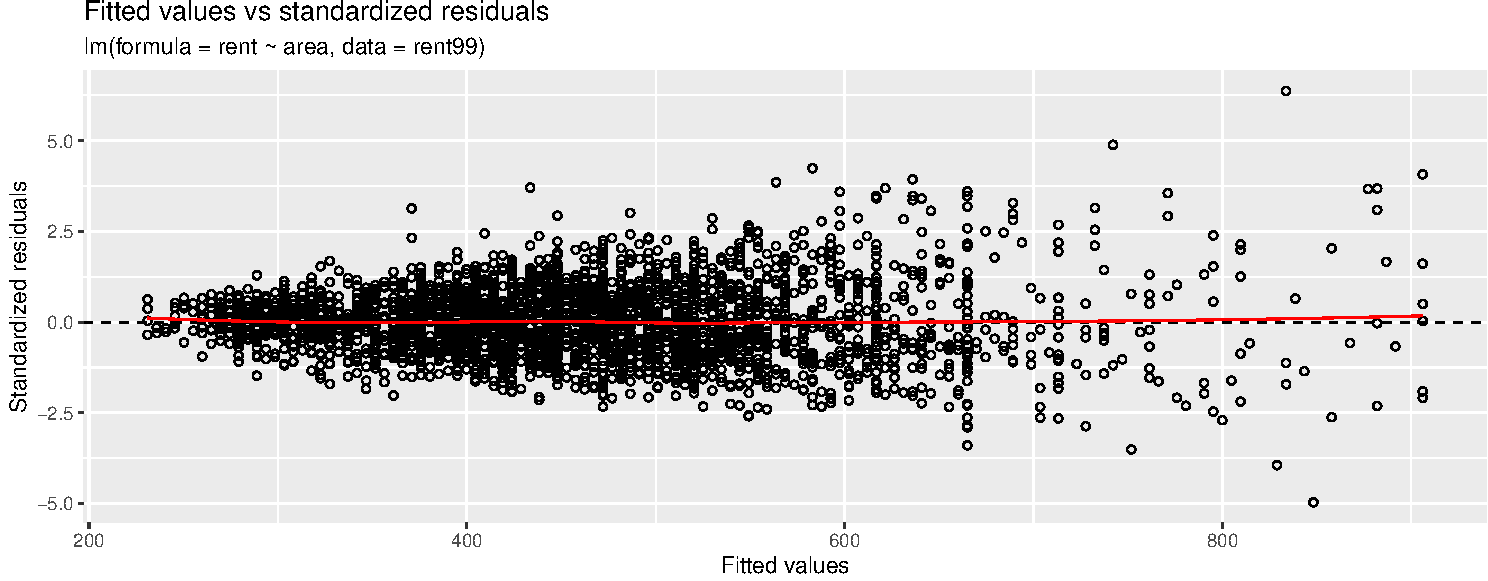
\includegraphics[keepaspectratio]{Module02MLRPresentationWeek1_files/figure-beamer/unnamed-chunk-7-1.pdf}}
\end{frame}

\begin{frame}[fragile]
\begin{block}{Normal Q-Q}
\phantomsection\label{normal-q-q}
This plot shows if the residuals are Gaussian (normally) distributed. If
they follow a straigt line it is an indication that they are, and else
they are probably not.

\begin{Shaded}
\begin{Highlighting}[]
\FunctionTok{ggplot}\NormalTok{(fit, }\FunctionTok{aes}\NormalTok{(}\AttributeTok{sample =}\NormalTok{ .stdresid)) }\SpecialCharTok{+} \FunctionTok{stat\_qq}\NormalTok{(}\AttributeTok{pch =} \DecValTok{19}\NormalTok{) }\SpecialCharTok{+} \FunctionTok{geom\_abline}\NormalTok{(}\AttributeTok{intercept =} \DecValTok{0}\NormalTok{,}
    \AttributeTok{slope =} \DecValTok{1}\NormalTok{, }\AttributeTok{linetype =} \StringTok{"dotted"}\NormalTok{) }\SpecialCharTok{+} \FunctionTok{labs}\NormalTok{(}\AttributeTok{x =} \StringTok{"Theoretical quantiles"}\NormalTok{,}
    \AttributeTok{y =} \StringTok{"Standardized residuals"}\NormalTok{, }\AttributeTok{title =} \StringTok{"Normal Q{-}Q"}\NormalTok{, }\AttributeTok{subtitle =} \FunctionTok{deparse}\NormalTok{(fit}\SpecialCharTok{$}\NormalTok{call))}
\end{Highlighting}
\end{Shaded}

\pandocbounded{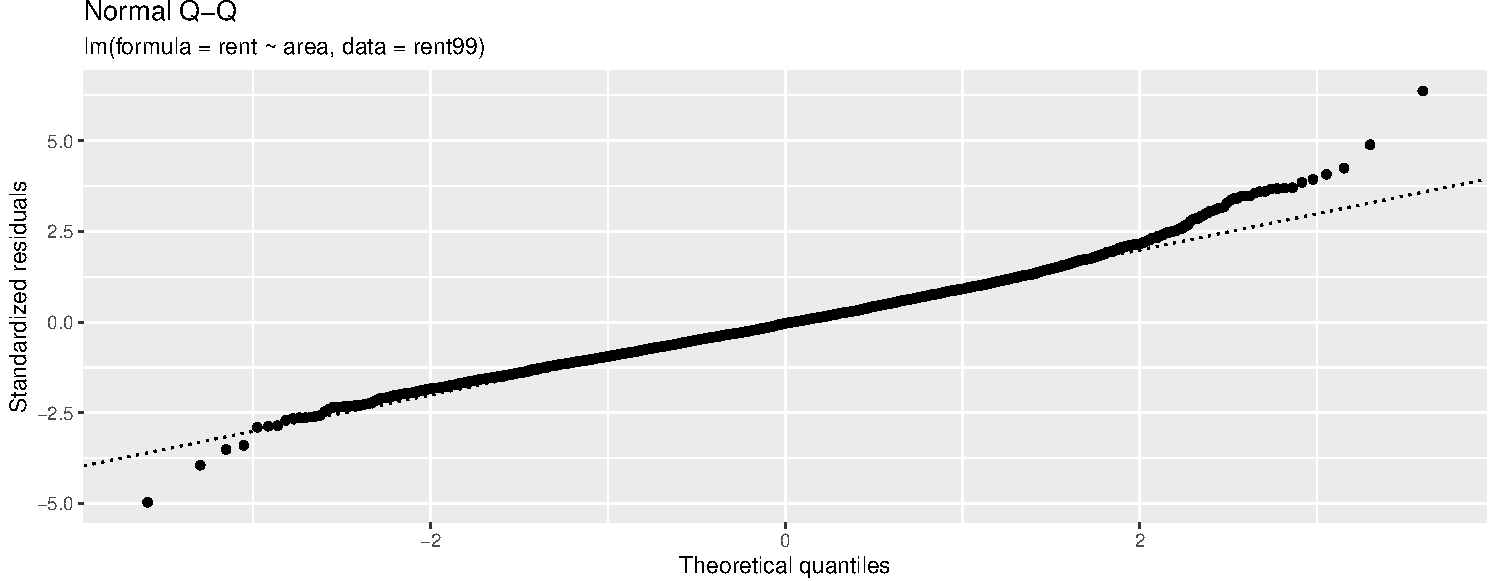
\includegraphics[keepaspectratio]{Module02MLRPresentationWeek1_files/figure-beamer/unnamed-chunk-8-1.pdf}}
\end{block}
\end{frame}

\begin{frame}
\begin{block}{Scale-location}
\phantomsection\label{scale-location}
This is also called spread-location plot. It shows if the residuals are
spread equally along the ranges of predictors. Can be used to check the
assumption of equal variance (homoscedasticity). A good plot is one with
a horizontal line with randomly spread points.

Is this plot good for your data?
\end{block}
\end{frame}

\begin{frame}[fragile]
\begin{Shaded}
\begin{Highlighting}[]
\FunctionTok{ggplot}\NormalTok{(fit, }\FunctionTok{aes}\NormalTok{(.fitted, }\FunctionTok{sqrt}\NormalTok{(}\FunctionTok{abs}\NormalTok{(.stdresid)))) }\SpecialCharTok{+} \FunctionTok{geom\_point}\NormalTok{() }\SpecialCharTok{+} \FunctionTok{geom\_smooth}\NormalTok{(}\AttributeTok{se =} \ConstantTok{FALSE}\NormalTok{,}
    \AttributeTok{col =} \StringTok{"red"}\NormalTok{, }\AttributeTok{size =} \FloatTok{0.5}\NormalTok{, }\AttributeTok{method =} \StringTok{"loess"}\NormalTok{) }\SpecialCharTok{+} \FunctionTok{labs}\NormalTok{(}\AttributeTok{x =} \StringTok{"Fitted values"}\NormalTok{,}
    \AttributeTok{y =} \FunctionTok{expression}\NormalTok{(}\FunctionTok{sqrt}\NormalTok{(}\StringTok{"Standardized residuals"}\NormalTok{)), }\AttributeTok{title =} \StringTok{"Scale{-}location"}\NormalTok{,}
    \AttributeTok{subtitle =} \FunctionTok{deparse}\NormalTok{(fit}\SpecialCharTok{$}\NormalTok{call))}
\end{Highlighting}
\end{Shaded}

\pandocbounded{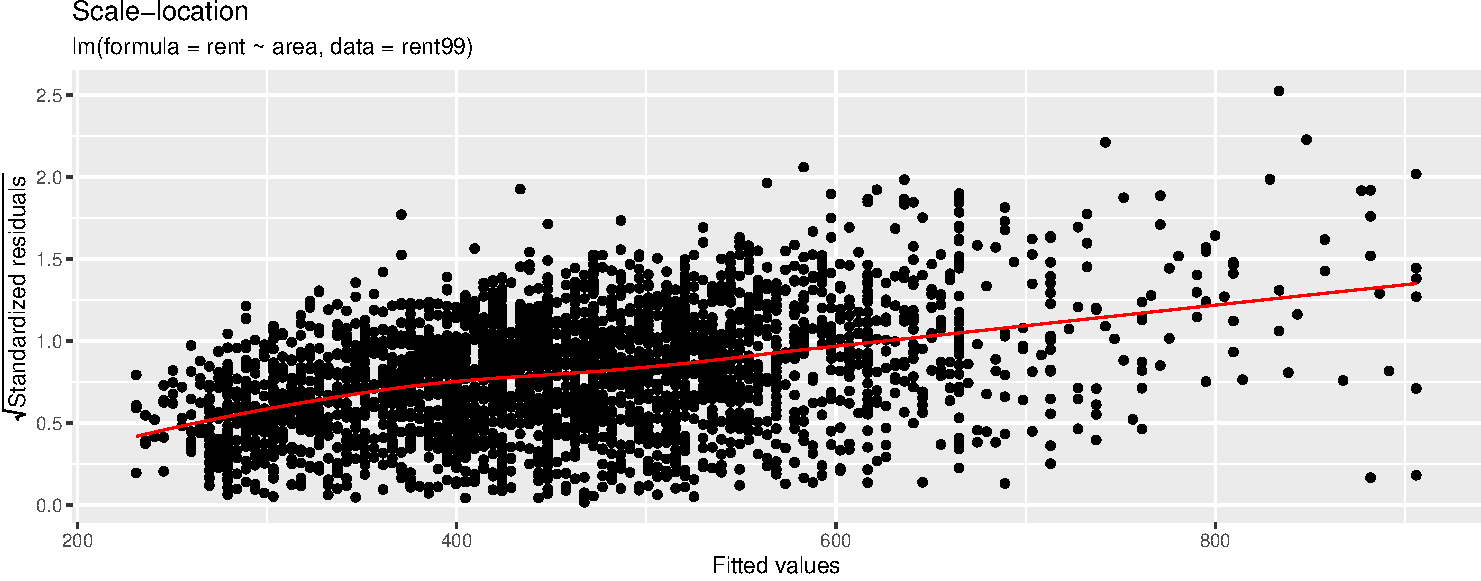
\includegraphics[keepaspectratio]{Module02MLRPresentationWeek1_files/figure-beamer/unnamed-chunk-9-1.pdf}}
\end{frame}

\begin{frame}
\begin{block}{Residual vs Leverage}
\phantomsection\label{residual-vs-leverage}
This plot can reveal influential outliers.

Not all outliers are influential in linear regression; the results might
not change if they are removed from the data set

Influential outliers can be seen as observations that does not get along
with the trend in the majority of the observations.
\end{block}
\end{frame}

\begin{frame}
Cook's distance is the Euclidean distance between the
\(\mathbf{\hat{y}}\) (the fitted values) and \(\mathbf{\hat{y}}_{(i)}\)
(the fitted values calculated when the \(i\)-th observation is omitted
from the regression).

This is then a measure on how much the model is influences by
observation \(i\).

The distance is scaled, and a rule of thumb is to examine observations
with Cook's distance larger than 1, and give some attention to those
with Cook's distance above 0.5.

Leverage is defined as the diagonal elements of the hat matrix, i.e.,
the leverage of the \(i\)-th data point is \(h_{ii}\) on the diagonal of
\(\mathbf{H = X(X^TX)^{-1}X^T}\). A large leverage indicated that the
observation (\(i\)) has a large influence on the estimation results, and
that the covariate values (\(\mathbf{x}_i\)) are unusual.
\end{frame}

\begin{frame}[fragile]
\begin{Shaded}
\begin{Highlighting}[]
\FunctionTok{ggplot}\NormalTok{(fit, }\FunctionTok{aes}\NormalTok{(.hat, .stdresid)) }\SpecialCharTok{+} \FunctionTok{geom\_smooth}\NormalTok{(}\AttributeTok{se =} \ConstantTok{FALSE}\NormalTok{, }\AttributeTok{col =} \StringTok{"red"}\NormalTok{,}
    \AttributeTok{size =} \FloatTok{0.5}\NormalTok{, }\AttributeTok{method =} \StringTok{"loess"}\NormalTok{) }\SpecialCharTok{+} \FunctionTok{geom\_point}\NormalTok{(}\FunctionTok{aes}\NormalTok{(}\AttributeTok{size =}\NormalTok{ .cooksd)) }\SpecialCharTok{+}
    \FunctionTok{scale\_size\_continuous}\NormalTok{(}\StringTok{"Cook\textquotesingle{}s dist."}\NormalTok{) }\SpecialCharTok{+} \FunctionTok{labs}\NormalTok{(}\AttributeTok{x =} \StringTok{"Leverage"}\NormalTok{, }\AttributeTok{y =} \StringTok{"Standardized residuals"}\NormalTok{,}
    \AttributeTok{title =} \StringTok{"Residuals vs Leverage"}\NormalTok{, }\AttributeTok{subtitle =} \FunctionTok{deparse}\NormalTok{(fit}\SpecialCharTok{$}\NormalTok{call))}
\end{Highlighting}
\end{Shaded}

\pandocbounded{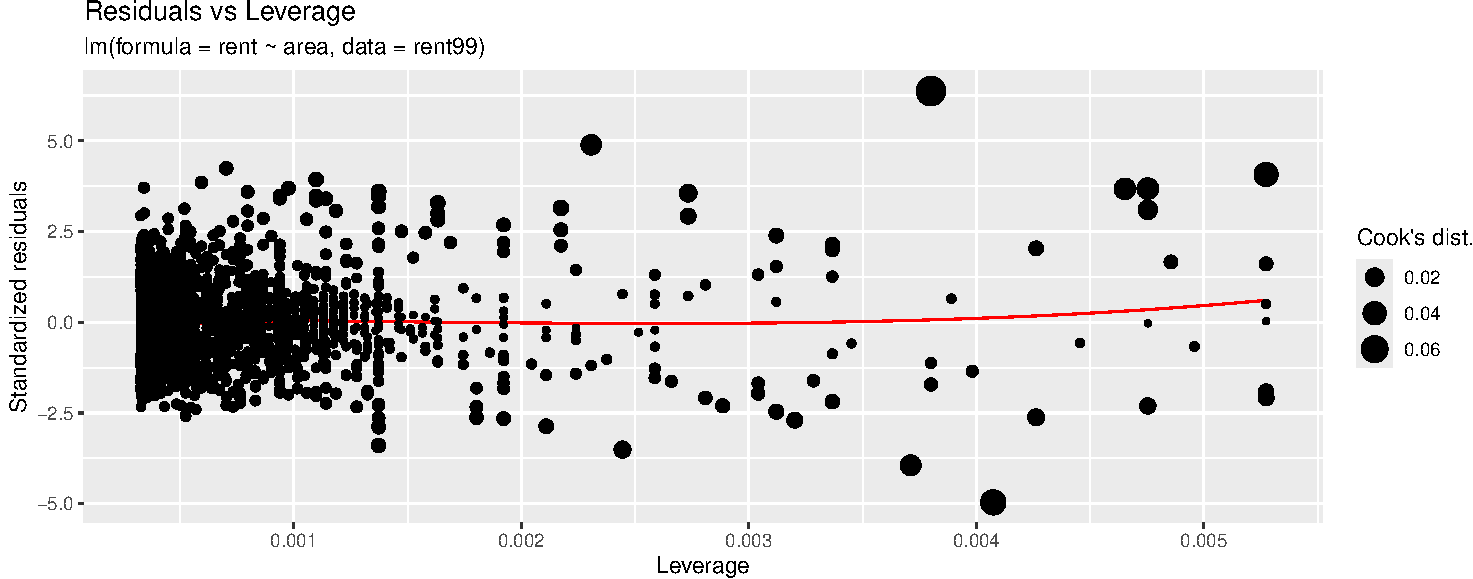
\includegraphics[keepaspectratio]{Module02MLRPresentationWeek1_files/figure-beamer/unnamed-chunk-10-1.pdf}}

(Some observations does not fit our model, but if we fit a more complex
model this may change.)
\end{frame}

\begin{frame}{Categorical covariates - dummy and effect coding}
\phantomsection\label{categorical-covariates---dummy-and-effect-coding}
(read for yourself - topic of ILw1)
\end{frame}

\begin{frame}[fragile]{Interactions}
\phantomsection\label{interactions}
(if we have time)

To illustrate how interactions between covariates can be included we use
the \texttt{ozone} data set from the \texttt{ElemStatLearn} library.
This data set is measurements from 1973 in New York and contains 111
observations of the following variables:

\begin{itemize}
\tightlist
\item
  \texttt{ozone} : ozone concentration (ppm)
\item
  \texttt{radiation} : solar radiation (langleys)
\item
  \texttt{temperature} : daily maximum temperature (F)
\item
  \texttt{wind} : wind speed (mph)
\end{itemize}
\end{frame}

\begin{frame}[fragile]{Ozone}
\phantomsection\label{ozone}
We start by fitting a multiple linear regression model to the data, with
\texttt{ozone} as our response variable and \texttt{temperature} and
\texttt{wind} as covariates.

\begin{longtable}[]{@{}rrrr@{}}
\toprule\noalign{}
ozone & radiation & temperature & wind \\
\midrule\noalign{}
\endhead
41 & 190 & 67 & 7.4 \\
36 & 118 & 72 & 8.0 \\
12 & 149 & 74 & 12.6 \\
18 & 313 & 62 & 11.5 \\
23 & 299 & 65 & 8.6 \\
19 & 99 & 59 & 13.8 \\
\bottomrule\noalign{}
\end{longtable}
\end{frame}

\begin{frame}[fragile]
\small

\begin{verbatim}
## 
## Call:
## lm(formula = ozone ~ temperature + wind, data = ozone)
## 
## Residuals:
##     Min      1Q  Median      3Q     Max 
## -42.160 -13.209  -3.089  10.588  98.470 
## 
## Coefficients:
##             Estimate Std. Error t value Pr(>|t|)    
## (Intercept) -67.2008    23.6083  -2.846  0.00529 ** 
## temperature   1.8265     0.2504   7.293 5.32e-11 ***
## wind         -3.2993     0.6706  -4.920 3.12e-06 ***
## ---
## Signif. codes:  0 '***' 0.001 '**' 0.01 '*' 0.05 '.' 0.1 ' ' 1
## 
## Residual standard error: 21.72 on 108 degrees of freedom
## Multiple R-squared:  0.5817, Adjusted R-squared:  0.574 
## F-statistic:  75.1 on 2 and 108 DF,  p-value: < 2.2e-16
\end{verbatim}

\normalsize
\end{frame}

\begin{frame}[fragile]
The model can be written as:
\[Y = \beta_0 + \beta_1 x_t + \beta_2 x_w + \varepsilon\] In this model
we have assumed that increasing the value of one covariate is
independent of the other covariates. For example: by increasing the
\texttt{temperature} by one-unit always increases the response value by
\(\beta_2 \approx 1.651\), regardless of the value of \texttt{wind}.
\end{frame}

\begin{frame}[fragile]
However, one might think that the covariate \texttt{wind} (wind speed)
might act differently upon \texttt{ozone} for different values of
\texttt{temperature} and vice verse. \[
\begin{aligned} Y &= \beta_0 +  \beta_1 x_t + \beta_2 x_w + \beta_3\cdot(x_t  \cdot x_w) +\varepsilon \\ 
&= \beta_0 +  (\beta_1 + \beta_3 x_w) \cdot x_t + \beta_2 x_w + \varepsilon \\ 
&= \beta_0 + \beta_1 x_t + (\beta_2 + \beta_3 x_t) \cdot x_w + \varepsilon \end{aligned}.
\] We fit this model in \texttt{R}. An interaction term can be included
in the model using the \texttt{*} symbol.

\textbf{Q:} Look at the \texttt{summary} below. Is this a better model
than without the interaction term? It the term significant?
\end{frame}

\begin{frame}[fragile]
\footnotesize

\begin{Shaded}
\begin{Highlighting}[]
\NormalTok{ozone.int }\OtherTok{=} \FunctionTok{lm}\NormalTok{(ozone }\SpecialCharTok{\textasciitilde{}}\NormalTok{ temperature }\SpecialCharTok{+}\NormalTok{ wind }\SpecialCharTok{+}\NormalTok{ temperature }\SpecialCharTok{*}\NormalTok{ wind, }\AttributeTok{data =}\NormalTok{ ozone)}
\FunctionTok{summary}\NormalTok{(ozone.int)}
\end{Highlighting}
\end{Shaded}

\begin{verbatim}
## 
## Call:
## lm(formula = ozone ~ temperature + wind + temperature * wind, 
##     data = ozone)
## 
## Residuals:
##     Min      1Q  Median      3Q     Max 
## -40.929 -11.190  -3.037   8.209  97.440 
## 
## Coefficients:
##                    Estimate Std. Error t value Pr(>|t|)    
## (Intercept)      -239.94146   48.59004  -4.938 2.92e-06 ***
## temperature         4.00151    0.59311   6.747 8.02e-10 ***
## wind               13.60882    4.28070   3.179  0.00193 ** 
## temperature:wind   -0.21747    0.05446  -3.993  0.00012 ***
## ---
## Signif. codes:  0 '***' 0.001 '**' 0.01 '*' 0.05 '.' 0.1 ' ' 1
## 
## Residual standard error: 20.36 on 107 degrees of freedom
## Multiple R-squared:  0.636,  Adjusted R-squared:  0.6258 
## F-statistic: 62.31 on 3 and 107 DF,  p-value: < 2.2e-16
\end{verbatim}

\normalsize
\end{frame}

\begin{frame}
Below we see that the interaction term is highly significant. The
\(p\)-value is very small, so that there is strong evidence that
\(\beta_3 \neq 0\). Furthermore, \(R^2_{\text{adj}}\) has increased,
indicating that more of the variability in the data has been explained
by the model (than without the interaction).
\end{frame}

\begin{frame}[fragile]
\emph{Interpretation of the interaction term:}

\begin{itemize}
\item
  If we now increase the \texttt{temperature} by \(10^{\circ}\) F, the
  increase in \texttt{wind} speed will be
  \[(\hat \beta_1+\hat \beta_3 \cdot x_w) \cdot 10 = (4.0 -0.22 \cdot x_w) \cdot 10 = 40-2.2 x_w \text{ units}.\]
\item
  If we increase the \texttt{wind} speed by 10 mph, the increase in
  \texttt{temperature} will be
  \[(\hat \beta_2 + \hat \beta_3 \cdot x_t) \cdot 10 = (14 -0.22 \cdot x_t) \cdot 10 = 140-2.2 x_t \text{ units}.\]
\end{itemize}
\end{frame}

\begin{frame}[fragile]
\begin{block}{The hierarchical principle}
\phantomsection\label{the-hierarchical-principle}
It is possible that the interaction term is highly significant, but the
main effects are not.

In our \texttt{ozone.int} model above: the main effects are
\texttt{temperature} and \texttt{wind}. The hierarchical principle
states that if we include an interaction term in our model, the main
effects are also to be included, even if they are not significant. This
means that if the coefficients \(\hat \beta_1\) or \(\hat \beta_2\)
would be insignificant, while the coefficient \(\hat \beta_3\) is
significant, \(\hat \beta_1\) and \(\hat \beta_2\) should still be
included in the model.
\end{block}
\end{frame}

\begin{frame}
\begin{block}{The hierarchical principle: why?}
\phantomsection\label{the-hierarchical-principle-why}
A model with interaction terms, but without the main effects is hard to
interpret.

Removing a main effect is the same as setting \(\beta_1=0\)

\[
Y = \beta_0 +  \beta_1 x_t + \beta_2 x_w + \beta_3\cdot(x_t  \cdot x_w) +\varepsilon
\]

i.e.~saying the slope of the \(x_t\) effect is 0 when \(x_w = 0\).
\end{block}
\end{frame}

\begin{frame}[fragile]
\begin{block}{Interactions between qualitative (discrete) and
quantitative (continuous) covariates}
\phantomsection\label{interactions-between-qualitative-discrete-and-quantitative-continuous-covariates}
We create a new variable \texttt{temp.cat} which is a
\texttt{temperature} as a qualitative covariate with two levels and fit
the model:
\[\begin{aligned}y&=\beta_0 + \beta_1 x_w + \begin{cases} \beta_2 + \beta_3  x_w  &\text{ if temperature="low"}\\ 0 &\text{ if temperature = "high"}\end{cases} \\\\ &= \begin{cases} (\beta_0 + \beta_2) + (\beta_1 + \beta_3) \cdot x_w &\text{ if temperature="low"}\\ \beta_0 + \beta_1 x_w &\text{ if temperature="high""} \end{cases} \end{aligned}\]
\end{block}
\end{frame}

\begin{frame}[fragile]{Ozone: make temperature categorical}
\phantomsection\label{ozone-make-temperature-categorical}
\begin{Shaded}
\begin{Highlighting}[]
\NormalTok{temp.cat }\OtherTok{=} \FunctionTok{ifelse}\NormalTok{(ozone}\SpecialCharTok{$}\NormalTok{temperature }\SpecialCharTok{\textless{}} \FunctionTok{mean}\NormalTok{(ozone}\SpecialCharTok{$}\NormalTok{temperature), }\StringTok{"low"}\NormalTok{,}
    \StringTok{"high"}\NormalTok{)}
\NormalTok{ozone2 }\OtherTok{=} \FunctionTok{cbind}\NormalTok{(ozone, temp.cat)}
\FunctionTok{kable}\NormalTok{(}\FunctionTok{head}\NormalTok{(ozone2))}
\end{Highlighting}
\end{Shaded}

\begin{longtable}[]{@{}rrrrl@{}}
\toprule\noalign{}
ozone & radiation & temperature & wind & temp.cat \\
\midrule\noalign{}
\endhead
41 & 190 & 67 & 7.4 & low \\
36 & 118 & 72 & 8.0 & low \\
12 & 149 & 74 & 12.6 & low \\
18 & 313 & 62 & 11.5 & low \\
23 & 299 & 65 & 8.6 & low \\
19 & 99 & 59 & 13.8 & low \\
\bottomrule\noalign{}
\end{longtable}
\end{frame}

\begin{frame}[fragile]{Model with interaction}
\phantomsection\label{model-with-interaction}
\begin{Shaded}
\begin{Highlighting}[]
\NormalTok{ozone.int2 }\OtherTok{=} \FunctionTok{lm}\NormalTok{(ozone }\SpecialCharTok{\textasciitilde{}}\NormalTok{ wind }\SpecialCharTok{+}\NormalTok{ temp.cat }\SpecialCharTok{+}\NormalTok{ temp.cat }\SpecialCharTok{*}\NormalTok{ wind, }\AttributeTok{data =}\NormalTok{ ozone2)}
\FunctionTok{summary}\NormalTok{(ozone.int2)}\SpecialCharTok{$}\NormalTok{coefficients}
\end{Highlighting}
\end{Shaded}

\begin{verbatim}
##                    Estimate Std. Error   t value     Pr(>|t|)
## (Intercept)      119.045026  7.5004384 15.871742 6.943657e-30
## wind              -6.723457  0.8195494 -8.203846 5.609913e-13
## temp.catlow      -92.631612 12.9465805 -7.154910 1.093470e-10
## wind:temp.catlow   6.054367  1.1999086  5.045690 1.860509e-06
\end{verbatim}
\end{frame}

\begin{frame}[fragile]
\begin{Shaded}
\begin{Highlighting}[]
\NormalTok{interceptlow }\OtherTok{=} \FunctionTok{coef}\NormalTok{(ozone.int2)[}\DecValTok{1}\NormalTok{] }\SpecialCharTok{+} \FunctionTok{coef}\NormalTok{(ozone.int2)[}\DecValTok{3}\NormalTok{]}
\NormalTok{slopelow }\OtherTok{=} \FunctionTok{coef}\NormalTok{(ozone.int2)[}\DecValTok{2}\NormalTok{] }\SpecialCharTok{+} \FunctionTok{coef}\NormalTok{(ozone.int2)[}\DecValTok{4}\NormalTok{]}
\NormalTok{intercepthigh }\OtherTok{=} \FunctionTok{coef}\NormalTok{(ozone.int2)[}\DecValTok{1}\NormalTok{]}
\NormalTok{slopehigh }\OtherTok{=} \FunctionTok{coef}\NormalTok{(ozone.int2)[}\DecValTok{2}\NormalTok{]}
\FunctionTok{ggplot}\NormalTok{(ozone) }\SpecialCharTok{+} \FunctionTok{geom\_line}\NormalTok{(}\FunctionTok{aes}\NormalTok{(}\AttributeTok{y =}\NormalTok{ interceptlow }\SpecialCharTok{+}\NormalTok{ slopelow }\SpecialCharTok{*}\NormalTok{ wind, }\AttributeTok{x =}\NormalTok{ wind),}
    \AttributeTok{col =} \StringTok{"blue"}\NormalTok{) }\SpecialCharTok{+} \FunctionTok{geom\_line}\NormalTok{(}\FunctionTok{aes}\NormalTok{(}\AttributeTok{y =}\NormalTok{ intercepthigh }\SpecialCharTok{+}\NormalTok{ slopehigh }\SpecialCharTok{*}\NormalTok{ wind,}
    \AttributeTok{x =}\NormalTok{ wind), }\AttributeTok{col =} \StringTok{"red"}\NormalTok{) }\SpecialCharTok{+} \FunctionTok{ylab}\NormalTok{(}\StringTok{"ozone"}\NormalTok{)}
\end{Highlighting}
\end{Shaded}

\pandocbounded{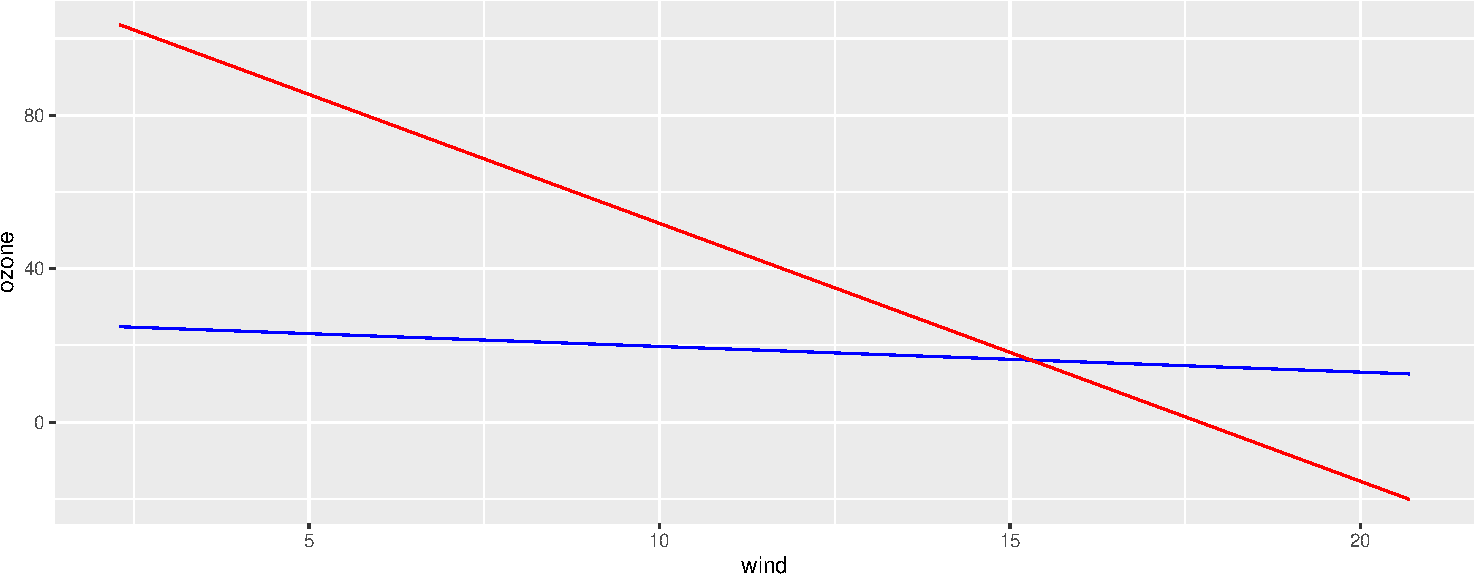
\includegraphics[keepaspectratio]{Module02MLRPresentationWeek1_files/figure-beamer/unnamed-chunk-16-1.pdf}}
\end{frame}

\end{document}
